\documentclass[a4paper]{article}

\usepackage{fontspec}
\setmainfont{Maple Mono}
\setmonofont{Maple Mono}
\usepackage{geometry}
\usepackage{graphicx}
\usepackage{subcaption}
\usepackage{amsmath, amssymb}

\usepackage[usenames,dvipsnames,svgnames,table]{xcolor}
\usepackage{listings}
\usepackage{tikz}
\usetikzlibrary{calc,positioning,shapes,arrows,fit}
\usepackage{cite}

\usepackage{hyperref}
\hypersetup{
    colorlinks=true,
    citecolor=Teal,
    linkcolor=Teal,
    pdftitle={Kinone: A Deep Learning Framework from First Principles},
    pdfauthor={Kshitish Kumar Ratha},
    pdfsubject={Summer Research Project Report},
    bookmarksopen=true,
    bookmarksnumbered=true
}

\geometry{
    left=25mm, right=25mm, top=25mm, bottom=25mm,
    headheight=13.6pt
}

\graphicspath{{./images/}}
\DeclareGraphicsExtensions{.png,.pdf,.jpg}

\lstset{
    language=python,
    basicstyle=\footnotesize\ttfamily,
    breaklines=true,
    numbers=left,
    numberstyle=\tiny\color{gray},
    numbersep=5pt,
    showstringspaces=false,
    commentstyle=\color{ForestGreen},
    keywordstyle=\color{teal},
    stringstyle=\color{red},
    backgroundcolor=\color[rgb]{0.97,0.97,0.95},
    tabsize=2,
    captionpos=b,
    keepspaces=true
}

\newcommand{\acronym}[1]{\textsc{#1}}


\begin{document}
\title{\textbf{Kinone: A Deep Learning Framework from First Principles}}

\author{
 Name: Kshitish Kumar Ratha \\
 Registration Number: MS22174 \\
}

\date{\today}

\maketitle

\begin{abstract}

    This report details the design, implementation, and verification of Kinone\footnote{The complete source code for this project is available at: \url{https://github.com/pseudofractal/kinone}.}, a deep learning framework developed from first principles using the NumPy scientific computing library. Motivated by the desire to demystify the internal mechanics of production-grade machine learning systems, this project constructs a transparent and auditable alternative. The framework's foundation is a reverse-mode automatic differentiation engine that operates on a dynamically generated computational graph, enabling the precise calculation of gradients for arbitrary scalar objectives through backpropagation. Built upon this core is a modular library of standard neural network primitives, including convolution, pooling, and normalization layers. The expressive power of this library is demonstrated through complete implementations of canonical deep learning architectures, specifically ResNet and EfficientNet. To support the full lifecycle of a machine learning project, Kinone is furnished with a custom data handling pipeline, a suite of common optimization algorithms, and tooling for interoperability, highlighted by an exporter to the ONNX format. A cornerstone of the development process was a rigorous verification strategy, where the analytical gradient of every operation was validated against numerical approximations from finite-difference methods. The result is a fully functional framework that serves as a powerful educational tool and an experimental platform for research requiring complete algorithmic control.

\end{abstract}

\pagebreak

\tableofcontents

\pagebreak

\section{Introduction}

The field of deep learning has been fundamentally transformed by the availability of high-performance, open-source frameworks such as PyTorch \cite{paszke2019pytorch}, TensorFlow, and JAX. These libraries provide a high level of abstraction, enabling researchers and practitioners to design, train, and deploy complex neural network architectures with remarkable efficiency. This abstraction, however, while a catalyst for productivity, often obscures the fundamental mechanics that underpin gradient-based learning. The intricate processes of gradient computation, parameter updates, and memory management are handled by highly optimized, often opaque, backend engines. For many users, these core components remain a "black box."

\subsection{Motivation and Problem Statement}

While the productivity gains offered by modern frameworks are undeniable, a reliance on them without a foundational understanding of their inner workings can be a significant impediment to deep learning research and advanced application. When a model fails to train, or when a novel architecture requires a non-standard operation, a first-principles understanding of the underlying system becomes indispensable. The core motivation for the Kinone project stems from this educational and experimental imperative: to deconstruct the "black box" by building a deep learning framework from scratch.

The central problem this project addresses is not a deficiency in existing tools, but rather a need for a system that prioritizes transparency, auditability, and pedagogical value over raw computational performance. The goal is to create a framework where every mathematical transformation and algorithmic step is explicit and accessible. Such a system serves two primary purposes. First, it is an unparalleled educational tool, forcing a concrete understanding of abstract concepts like backpropagation and the chain rule by requiring their direct implementation. Second, it provides a scaffold for research experiments that demand complete algorithmic control and deterministic behavior, which can sometimes be challenging to guarantee in frameworks that rely on device-specific kernels and complex optimizations.

Kinone is the proposed solution to this problem. It is a self-contained deep learning framework implemented entirely in Python with NumPy as its sole numerical dependency. By deliberately avoiding external machine learning libraries, it ensures that the complete chain of logic—from the forward pass through a network to the backward pass of gradients—is contained and auditable within the project's own codebase.

\subsection{Project Goals and Scope}

To address the problem statement, the project was defined by a series of clear, concrete objectives. The successful completion of these goals resulted in the creation of a functional, end-to-end framework capable of handling a non-trivial machine learning task. The primary goals were as follows:

\begin{itemize}
    \item \textbf{To design and implement a reverse-mode automatic differentiation engine.} This core component, often called an "autograd" engine, needed to dynamically construct a computational graph and correctly propagate gradients from a scalar loss function back to every parameter in the model.

    \item \textbf{To build a comprehensive library of essential neural network layers and operations.} This involved creating robust and numerically stable implementations of standard primitives, including element-wise operations, matrix multiplication, 2D convolutions, pooling, and normalization layers.

    \item \textbf{To implement canonical deep learning architectures.} To validate the framework's expressive power and modularity, well-known models such as ResNet and EfficientNet were implemented using the developed library of layers.

    \item \textbf{To develop a complete data handling and training pipeline.} This encompassed creating a dataset-specific loader for a real-world dataset (NIH Chest X-ray), implementing standard optimization algorithms like Adam and SGD, and structuring a training script to manage the learning process.

    \item \textbf{To ensure correctness through a rigorous and systematic testing strategy.} A cornerstone of the project was to guarantee the correctness of the autograd engine. This was achieved by creating a full suite of unit tests where the analytically derived gradient for every operation was verified against a numerical approximation calculated using the finite-difference method.

    \item \textbf{To create supporting tools for analysis and interoperability.} To make the framework a more complete ecosystem, an ONNX exporter was developed to allow models to be used in other environments, and a Streamlit-based dashboard was created for monitoring the training process.

    \item \textbf{To run inference on edge-devices.} The ONNX export needs to be quantized by and then run inference on an AMD-Xilinx Kria KV260 Vision AI Starter Kit to showcase the efficiency of the architecture and the framework's ability to deploy models on resource-constrained devices.
\end{itemize}

The scope of this project was intentionally focused on correctness, clarity, and architectural completeness rather than computational performance. No GPU acceleration or low-level performance optimization was attempted. Kinone is therefore positioned as an educational and experimental tool, not as a performance-competitive replacement for production frameworks.

\subsection{Report Structure}

The remainder of this report is organized as follows. Section 2 reviews the theoretical foundations of automatic differentiation and gradient-based optimization that form the basis of the framework. Section 3 provides a detailed architectural overview and implementation details of the Kinone framework, from the core autograd engine to the high-level model definitions. Section 4 describes the verification and testing strategy used to ensure the correctness of the gradient calculations. Finally, Section 5 concludes the report with a summary of the project's achievements, key learnings, and potential directions for future work.

\section{Theoretical Foundations}

The implementation of the Kinone framework is predicated on a set of foundational mathematical and algorithmic principles that together enable modern gradient-based learning. This section provides a review of these core concepts, from the abstract representation of computation to the specific algorithms used for network optimization. Understanding these principles is essential for appreciating the design decisions made throughout the framework's architecture.

\subsection{The Computational Graph}

At its core, any differentiable program, from a simple arithmetic expression to a deep neural network, can be decomposed into a sequence of elementary operations. This decomposition can be formally represented as a Directed Acyclic Graph (\acronym{dag}), commonly known as a computational graph. In this graph, nodes represent either variables (e.g., tensors containing data, parameters, or intermediate values) or operations (e.g., matrix multiplication, addition, activation functions). The directed edges represent the flow of data, connecting the variables that serve as inputs to an operation, and connecting the operation to its resulting output variable.

Kinone adheres to the \textit{define-by-run} paradigm, a concept popularized by frameworks like Chainer and PyTorch \cite{paszke2019pytorch}. This means the computational graph is not statically declared beforehand but is built dynamically as the forward pass is executed. Each time an operation is applied to one or more tensors, a new output tensor is created, and a new node representing the operation is implicitly added to the graph. This operation node retains pointers to its input tensors (its "parents") and the output tensor (its "child").

This dynamic graph structure is not merely a conceptual model; it is the central data structure upon which the entire process of automatic differentiation rests. By recording the precise sequence of operations and their data dependencies, the graph provides a complete roadmap for the backward pass, ensuring that gradients can be correctly propagated back through the network from the final loss to every contributing parameter. Figure \ref{fig:comp_graph_nn} illustrates a simple computational graph for a single neuron.

\begin{figure}[h!]
    \centering
    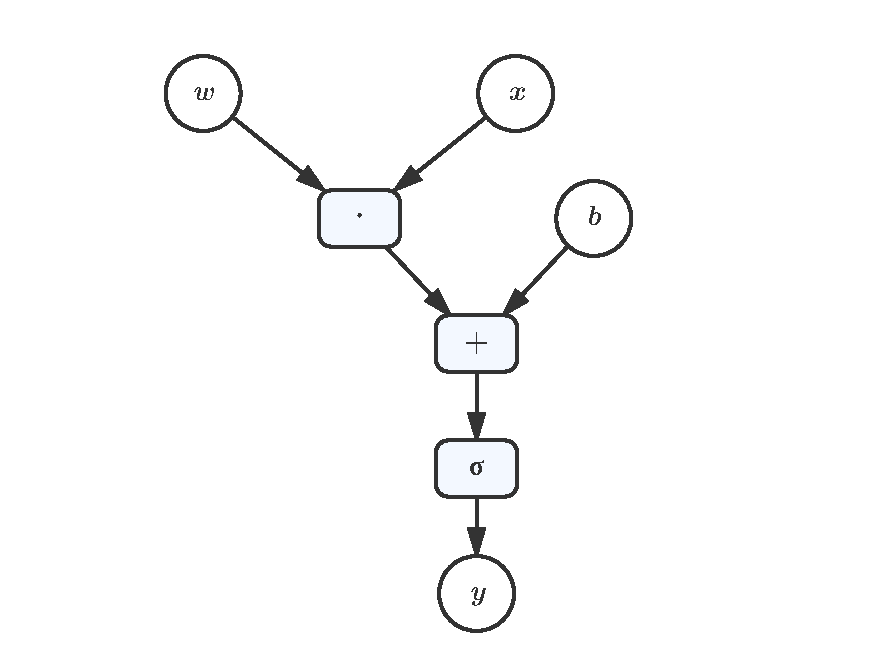
\includegraphics[width=0.7\textwidth]{comp_graph_nn}
    \caption{Computational Graph for a Single Neuron: \(y = \sigma(\mathbf{w}\cdot \mathbf{x} + b)\)}
    \label{fig:comp_graph_nn}
\end{figure}

\subsection{Reverse-Mode Automatic Differentiation}

Automatic Differentiation (\acronym{ad}) is a family of techniques for numerically evaluating the derivative of a function specified by a computer program. For training deep neural networks, the preferred technique is reverse-mode \acronym{ad}, commonly known as backpropagation \cite{rumelhart1986learning}. Its goal is to efficiently compute the gradient of a single scalar output (the loss, $\mathcal{L}$) with respect to a large number of input variables (the model parameters, $\theta$).

The mathematical foundation of backpropagation is the multivariable chain rule. Consider a simple composition of vector functions, where a final scalar loss $\mathcal{L}$ is computed via an intermediate variable $\mathbf{u}$:
\begin{equation}
    \mathbf{u} = g(\mathbf{v}) \quad \text{and} \quad \mathcal{L} = f(\mathbf{u})
\end{equation}
The chain rule states that the derivative of the loss $\mathcal{L}$ with respect to the input $\mathbf{v}$ can be expressed using the Jacobian matrices of the functions $f$ and $g$:
\begin{equation}
    \frac{\partial \mathcal{L}}{\partial \mathbf{v}} = \frac{\partial \mathcal{L}}{\partial \mathbf{u}} \frac{\partial \mathbf{u}}{\partial \mathbf{v}} = \nabla_{\mathbf{u}} \mathcal{L} \cdot J_g(\mathbf{v})
\end{equation}
where $J_g(\mathbf{v})$ is the Jacobian of $g$ evaluated at $\mathbf{v}$, and $\nabla_{\mathbf{u}} \mathcal{L}$ is the gradient of $\mathcal{L}$ with respect to $\mathbf{u}$.

Reverse-mode \acronym{ad} applies this rule by traversing the computational graph backward, from the final output node to the input nodes. At each operation node, it computes the gradient with respect to that node's inputs based on the gradient it has already received from its output (the "upstream gradient"). If we denote the gradient of the final loss $\mathcal{L}$ with respect to a tensor $\mathbf{x}$ as $\bar{\mathbf{x}} = \nabla_{\mathbf{x}} \mathcal{L}$, the core update rule for an operation $\mathbf{u} = g(\mathbf{v})$ is:
\begin{equation}
    \bar{\mathbf{v}} = J_g(\mathbf{v})^{\top} \bar{\mathbf{u}}
\end{equation}

\begin{figure}[t]
  \centering
  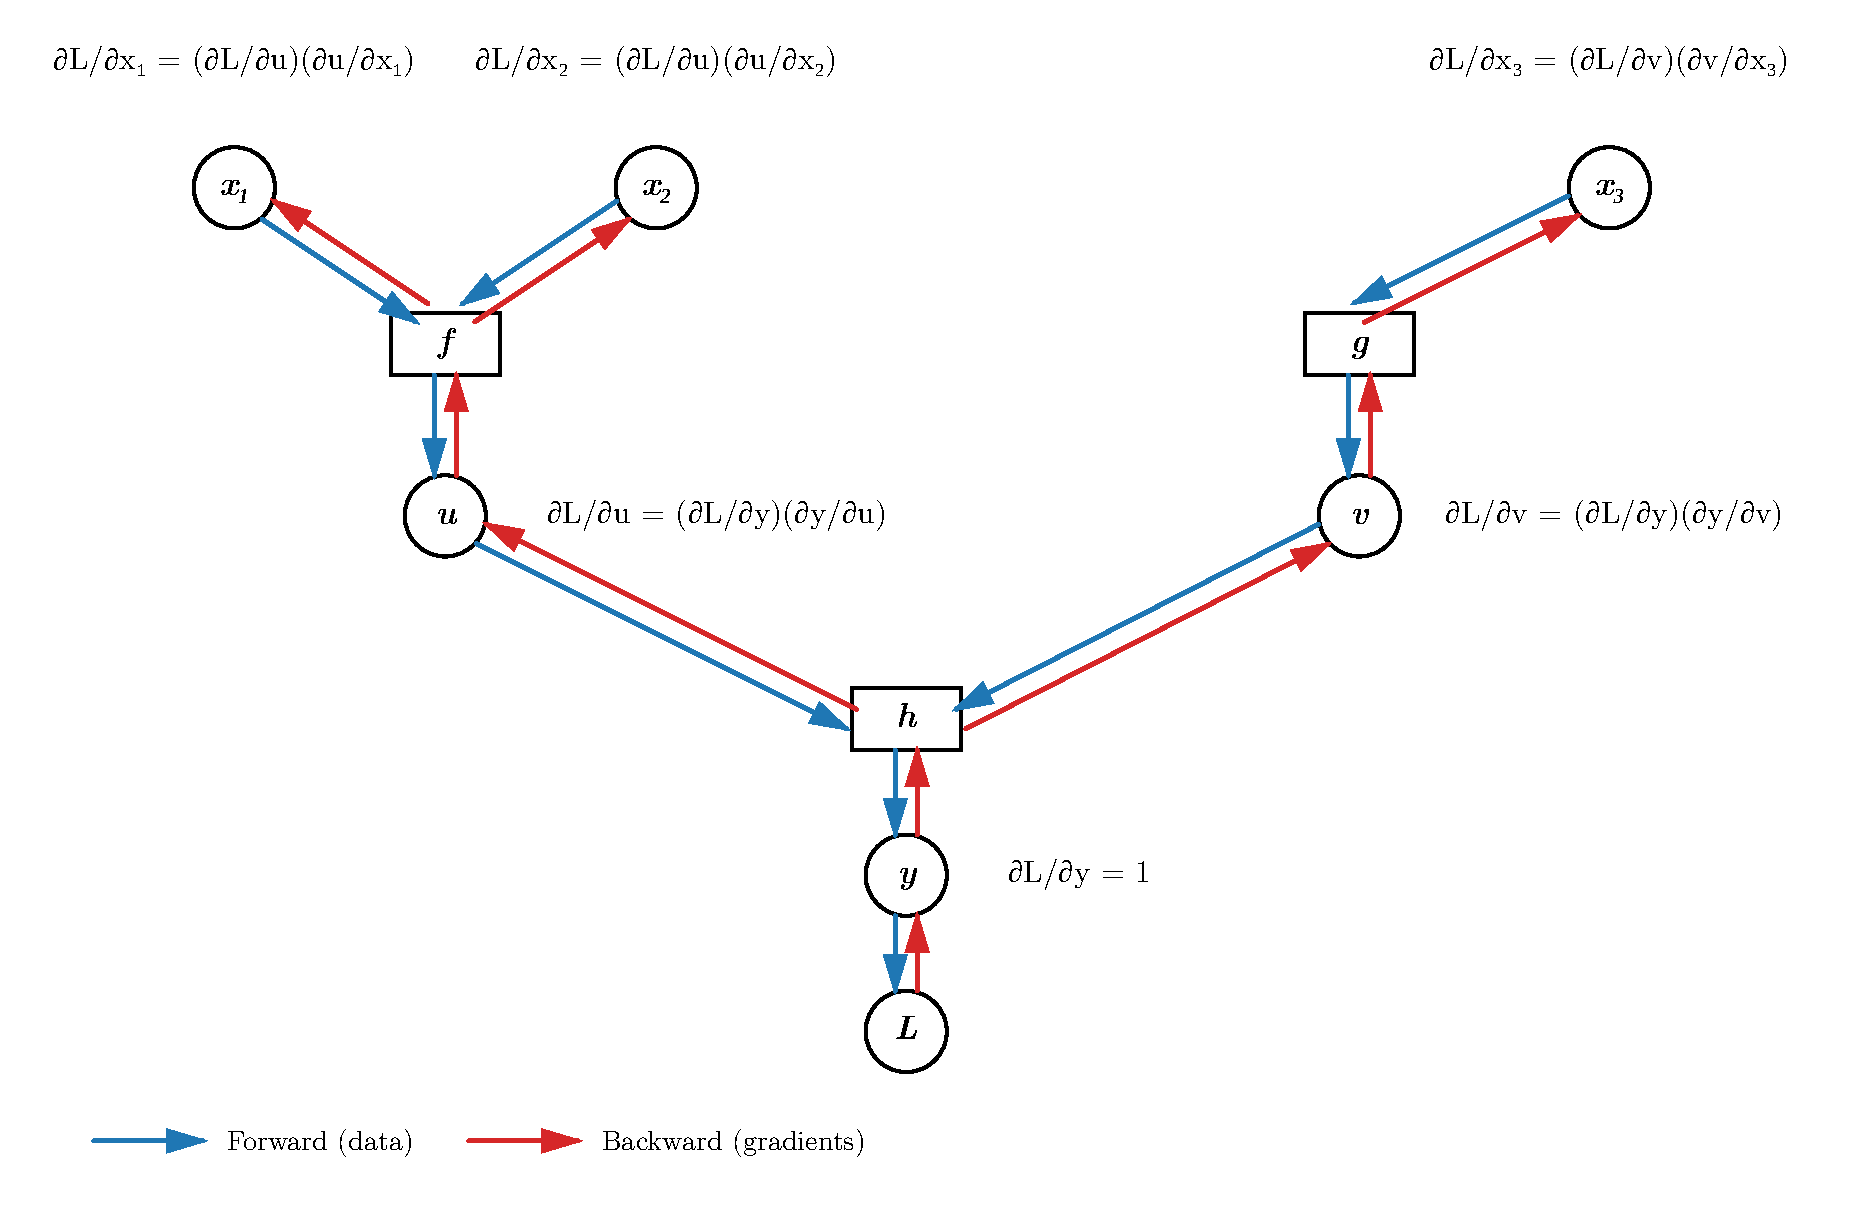
\includegraphics[width=0.8\textwidth]{rev_ad_diagram}
  \caption{Reverse-mode AD on a small computational graph. Solid black arrows
  show the forward data flow; dashed red arrows show the backward gradient
  sweep, applying vector–Jacobian products \( \partial \mathcal{L}/\partial u
  = (\partial \mathcal{L}/\partial y)(\partial y/\partial u) \), etc.}
  \label{fig:rev_ad_mechanics}
\end{figure}

This process begins by initializing the gradient of the loss with respect to itself to one ($\bar{\mathcal{L}} = 1$). The algorithm then proceeds in reverse topological order of the graph, applying this update rule at each node. A key detail is that if a variable is used in multiple subsequent operations, its total gradient is the sum of the gradients propagated back from each of those branches.

This method is exceptionally efficient for deep learning because it calculates the gradients for all parameters in a single backward pass through the graph, with a computational cost that is a small constant multiple of the forward pass. Kinone's `Tensor.backward()` method is a direct implementation of this algorithm, performing a depth-first search to establish the topological order before accumulating gradients.

\subsection{Neural Network Primitives}

The power of a deep learning framework comes from its library of pre-defined, differentiable operations that can be composed to form complex models. The following are key primitives implemented in Kinone.

\subsubsection{2D Convolution}
The 2D convolution is the cornerstone of modern computer vision models, famously used in pioneering architectures such as LeNet-5 \cite{lecun1998gradient}. It operates by sliding a small, learnable kernel (or filter) over the spatial dimensions of a multi-channel input tensor. At each position, it computes the dot product between the kernel's weights and the corresponding input patch. For an input tensor $\mathbf{X}$ and a kernel $\mathbf{W}$, the output $\mathbf{Y}$ is given by:
\begin{equation}
    Y_{n, c_{out}, i, j} = b_{c_{out}} + \sum_{c_{in}=0}^{C_{in}-1} \sum_{k=0}^{K-1} \sum_{l=0}^{L-1} X_{n, c_{in}, i \cdot s + k, j \cdot s + l} \cdot W_{c_{out}, c_{in}, k, l}
\end{equation}
where $s$ is the stride and $b$ is an optional bias term. This operation allows the model to learn hierarchical spatial features, such as edges, textures, and eventually complex objects.

\subsubsection{Batch Normalization}
Batch Normalization is a critical technique for stabilizing and accelerating the training of deep networks \cite{ioffe2015batch}. It normalizes the output of a previous layer by subtracting the mini-batch mean and dividing by the mini-batch standard deviation. The normalized output is then scaled and shifted by two learnable parameters, $\gamma$ (gamma) and $\beta$ (beta). For a mini-batch of activations $\mathcal{B} = \{x_1, \dots, x_m\}$, the operation for each activation $x_i$ is:
\begin{align*}
    \mu_{\mathcal{B}} &= \frac{1}{m} \sum_{i=1}^{m} x_i \quad (\text{mini-batch mean}) \\
    \sigma^2_{\mathcal{B}} &= \frac{1}{m} \sum_{i=1}^{m} (x_i - \mu_{\mathcal{B}})^2 \quad (\text{mini-batch variance}) \\
    \hat{x}_i &= \frac{x_i - \mu_{\mathcal{B}}}{\sqrt{\sigma^2_{\mathcal{B}} + \epsilon}} \quad (\text{normalize}) \\
    y_i &= \gamma \hat{x}_i + \beta \quad (\text{scale and shift})
\end{align*}
During inference, the mean and variance are not computed per-batch but are instead replaced by running averages of these statistics collected during training. The backward pass for this operation is non-trivial, as the gradient for each sample depends on all other samples in the mini-batch.

\subsection{Gradient-Based Optimization}

Once the gradients of the loss function with respect to all model parameters ($\nabla_{\theta} \mathcal{L}$) have been computed, an optimizer uses these gradients to update the parameters in a direction that is expected to minimize the loss. All optimizers follow a general update rule:
\begin{equation}
    \theta_{t+1} \leftarrow \theta_t - \eta \cdot \Delta \theta_t
\end{equation}
where $\theta_t$ are the parameters at timestep $t$, $\eta$ is the learning rate, and $\Delta \theta_t$ is the update step derived from the gradients. Kinone implements several standard algorithms.

\subsubsection{Stochastic Gradient Descent (SGD)}
The simplest optimizer, SGD, uses the raw gradient as the update direction: $\Delta \theta_t = \nabla_{\theta_t} \mathcal{L}(\theta_t)$. A common extension is SGD with momentum, which introduces a velocity term $\mathbf{v}_t$ that accumulates an exponentially decaying moving average of past gradients. This helps to dampen oscillations and accelerate convergence along persistent directions. The update rules are:
\begin{align*}
    \mathbf{v}_{t+1} &\leftarrow \mu \mathbf{v}_t + \nabla_{\theta_t} \mathcal{L}(\theta_t) \\
    \theta_{t+1} &\leftarrow \theta_t - \eta \mathbf{v}_{t+1}
\end{align*}
where $\mu$ is the momentum coefficient.

\subsubsection{Adaptive Optimizers: RMSProp and Adam}
Adaptive methods adjust the learning rate for each parameter individually. \textbf{RMSProp} \cite{hinton2012neural} maintains a moving average of the squared gradients for each parameter and divides the learning rate by the square root of this average. This effectively decreases the learning rate for parameters with large, consistent gradients and increases it for parameters with small or infrequent gradients.

\textbf{Adam (Adaptive Moment Estimation)} is arguably the most common optimizer in modern deep learning \cite{kingma2014adam}. It combines the ideas of momentum (the first moment of the gradients) and per-parameter adaptive learning rates (the second moment of the gradients). It maintains two moving averages for each parameter:
\begin{align*}
    m_t &= \beta_1 m_{t-1} + (1 - \beta_1) g_t \quad (\text{first moment estimate}) \\
    v_t &= \beta_2 v_{t-1} + (1 - \beta_2) g_t^2 \quad (\text{second moment estimate})
\end{align*}
where $g_t = \nabla_{\theta_t} \mathcal{L}$. Adam also includes a bias-correction step to account for the fact that these estimates are initialized at zero. The final parameter update is then:
\begin{equation}
    \theta_{t+1} \leftarrow \theta_t - \eta \frac{\hat{m}_t}{\sqrt{\hat{v}_t} + \epsilon}
\end{equation}
where $\hat{m}_t$ and $\hat{v}_t$ are the bias-corrected moment estimates. This combination provides a robust and efficient optimization algorithm that works well across a wide range of problems.

\section{Framework Architecture and Implementation}

The Kinone framework is designed as a layered system, with each layer of abstraction building upon the one below it. This modular design promotes code reuse, simplifies debugging, and maintains a clear separation of concerns. This section provides a comprehensive overview of the framework's architecture, starting from the core automatic differentiation engine and progressing to the high-level model implementations and supporting tools.

\subsection{The Core Autograd Engine}

The engine, located in \texttt{src/core/}, is the cornerstone of the framework. It is responsible for constructing the computational graph and performing backpropagation. It consists of two primary classes: \texttt{Tensor} and \texttt{Function}.

\subsubsection{The \texttt{Tensor} Class}

The \texttt{Tensor} class, defined in \texttt{src/core/tensor.py}, is the fundamental data structure in Kinone. It serves as a wrapper around a NumPy \texttt{ndarray} and acts as a node in the computational graph. Its primary responsibilities are to store the raw data, track whether gradients are required, and accumulate gradients during the backward pass. The key attributes of a \texttt{Tensor} are:

\begin{itemize}
    \item \texttt{data}: The underlying \texttt{np.ndarray} that holds the numerical data.
    \item \texttt{requires\_grad}: A boolean flag indicating whether this tensor is a parameter or an intermediate value that requires a gradient to be computed for it.
    \item \texttt{grad}: A \texttt{Tensor} object that stores the accumulated gradient. It is initialized to \texttt{None} and is populated during the backward pass.
    \item \texttt{\_ctx}: A reference to a \texttt{Function} object that created this tensor. This is the link that forms the backward graph, pointing to the operation that generated this tensor. For user-created tensors (leaf nodes), this is \texttt{None}.
\end{itemize}

By overloading standard arithmetic operators (e.g., \texttt{\_\_add\_\_}, \texttt{\_\_mul\_\_}), the \texttt{Tensor} class provides a seamless and intuitive API for building the computational graph.

\subsubsection{The \texttt{Function} Abstraction}

Every operation in the graph is an instance of a class that inherits from the abstract base class \texttt{Function}, defined in \texttt{src/core/ops.py}. This class provides the machinery for both the forward and backward passes of an operation. Its design is centered around a single class method, \texttt{apply}, which orchestrates the graph construction.

\begin{lstlisting}[caption={The \texttt{Function.apply} method orchestrates graph construction.}, label={lst:function_apply}]
@classmethod
def apply(cls, *args, **kwargs) -> Tensor:
  context = cls()
  context.parents = [arg for arg in args if isinstance(arg, Tensor)]
  
  raw_args = [arg.data if isinstance(arg, Tensor) else arg for arg in args]
  output_data = cls.forward(context, *raw_args, **kwargs)
  
  requires_grad = any(p.requires_grad for p in context.parents)
  output_tensor = Tensor(output_data, requires_grad)
  output_tensor._ctx = context if requires_grad else None
  
  return output_tensor
\end{lstlisting}

When an operation like \texttt{add(a, b)} is called, it internally invokes \texttt{Add.apply(a, b)}. This method performs several critical steps:
\begin{enumerate}
    \item It instantiates the specific function class (e.g., \texttt{Add}), creating a \texttt{context} object.
    \item It saves the input tensors (\texttt{a} and \texttt{b}) as \texttt{context.parents}.
    \item It calls the static \texttt{forward} method with the raw NumPy data to compute the result.
    \item It creates a new output \texttt{Tensor} to hold the result.
    \item Crucially, it sets the \texttt{\_ctx} attribute of the new output tensor to the \texttt{context} object, thereby linking the output to the operation and inputs that created it.
\end{enumerate}

Each concrete \texttt{Function} subclass must implement two methods: \texttt{forward}, which defines the mathematical computation, and \texttt{backward}, which defines the analytical derivative (the vector-Jacobian product) for that operation.

\subsubsection{The Backpropagation Algorithm}

The backpropagation process is initiated by calling the \texttt{backward()} method on the final scalar tensor (typically the loss). This method, implemented in \texttt{src/core/tensor.py}, executes the reverse-mode automatic differentiation algorithm described in Section 2.2. The implementation proceeds in two main phases:

\begin{enumerate}
    \item \textbf{Topological Sort:} First, a correct processing order for the backward pass must be established. The graph is traversed from the final node backwards using a depth-first search (\acronym{dfs}), and nodes are added to a list in post-order. This effectively creates a reverse topological sort of the graph, ensuring that when we process a node, we have already processed all of its successors.

    \item \textbf{Gradient Accumulation:} The algorithm then iterates through the sorted list of nodes in reverse. For each tensor in the list, it accesses its \texttt{\_ctx} (the \texttt{Function} that created it). It then calls the \texttt{backward} method of that \texttt{Function}, passing the upstream gradient that has been accumulated in the current tensor's \texttt{.grad} attribute. The \texttt{backward} method returns the local gradients with respect to each of its inputs. These local gradients are then accumulated into the \texttt{.grad} attributes of the parent tensors.
\end{enumerate}

This process continues until all nodes in the graph that contributed to the final output have been visited, at which point the \texttt{.grad} attribute of every parameter tensor contains the complete gradient of the loss with respect to that parameter.

\subsection{Library of Operations}

Building on the \texttt{Function} abstraction, Kinone implements a wide array of differentiable operations in \texttt{src/core/ops.py}. These primitives are the fundamental building blocks for all layers and models.

\begin{table}[h!]
 \centering
 \caption{A Selection of Implemented Primitive Operations} \label{tab:ops}
 \begin{tabular}{|l|l|}
  \hline
  \textbf{Category} & \textbf{Operators} \\ \hline
  Element-wise & \texttt{Add}, \texttt{Sub}, \texttt{Mul}, \texttt{Div}, \texttt{Neg} \\
  Activations & \texttt{ReLU}, \texttt{Sigmoid}, \texttt{Tanh}, \texttt{Swish}, \texttt{HardSigmoid}, \texttt{HardSwish} \\
  Reductions & \texttt{Sum}, \texttt{Mean} \\
  Linear Algebra & \texttt{MatMul} \\
  Convolutions & \texttt{Conv2d}, \texttt{ConvNd}, \texttt{ConvTransposeNd} \\ \hline
 \end{tabular}
\end{table}

A notable implementation detail is the handling of convolution. To maintain efficiency without relying on external libraries, the \texttt{Conv2d} operation uses the \texttt{im2col} (image-to-column) technique. This method transforms the local patches of the input image into columns of a large matrix. The convolution operation can then be reformulated as a single, highly optimized matrix multiplication between this matrix and the reshaped convolution kernels. The backward pass is implemented via the corresponding \texttt{col2im} operation. Furthermore, a utility function, \texttt{\_unbroadcast}, was implemented to correctly handle the backward pass for operations involving NumPy broadcasting, ensuring that gradients are correctly summed over the broadcasted dimensions.

\subsection{Neural Network Modules}

To facilitate the construction of complex models, Kinone provides a higher level of abstraction through its \texttt{Module} system, located in \texttt{src/core/modules.py}, \texttt{pool.py}, and \texttt{batchnorm.py}. This system is heavily inspired by the design of PyTorch.

\subsubsection{The \texttt{Module} Base Class}

The \texttt{Module} class is the base class for all neural network layers. It provides essential functionality for managing a layer's state and parameters:
\begin{itemize}
    \item \textbf{Parameter Tracking:} It automatically registers any attributes that are instances of \texttt{Tensor} or other \texttt{Module}s as part of its state. The \texttt{parameters()} and \texttt{named\_parameters()} methods provide convenient iterators for accessing all parameters within a module and its sub-modules, which is essential for passing them to an optimizer.
    \item \textbf{State Management:} It maintains a \texttt{training} attribute to switch between training and evaluation modes. This is critical for layers like \texttt{BatchNorm2d} and \texttt{Dropout} that behave differently in each mode.
    \item \textbf{Serialization:} The \texttt{load\_state\_dict} method allows for loading pre-trained weights from a dictionary, enabling model checkpointing and inference.
\end{itemize}

\subsubsection{Layer Implementations}

Specific layers are implemented as subclasses of \texttt{Module}. They encapsulate the parameters and the forward pass logic for a common neural network operation.
\begin{itemize}
    \item \texttt{Linear}: Implements a fully connected layer. It initializes weight and bias tensors and its forward pass is defined as a composition of the primitive \texttt{matmul} and \texttt{add} operations.
    \item \texttt{Conv2D}: Encapsulates a 2D convolution. It holds the kernel and bias tensors as parameters and calls the \texttt{conv2d} primitive function in its forward pass.
    \item \texttt{BatchNorm2d}: Implements 2D batch normalization. It manages the learnable \texttt{gamma} and \texttt{beta} parameters as well as the non-learnable \texttt{running\_mean} and \texttt{running\_var} buffers.
    \item \texttt{Sequential}: A container module that chains a sequence of other modules together, allowing for the easy construction of feed-forward network blocks.
\end{itemize}

\subsection{Model Architectures}

The modular design of the framework culminates in the ability to construct complex, state-of-the-art model architectures, which are defined in \texttt{src/core/models/}.

\subsubsection{ResNet Implementation}
The implementation of the ResNet family of models (\texttt{resnet.py}) demonstrates the framework's ability to handle one of the most influential architectures in computer vision \cite{he2016deep}. It includes implementations of the \texttt{BasicBlock} and \texttt{Bottleneck} residual blocks. The critical skip connection is implemented simply by adding the block's input to its output using the framework's \texttt{add} operation before the final activation function, showcasing the power of the underlying computational graph.

\subsubsection{EfficientNet Implementation}
To further test the framework's capabilities, a version of the EfficientNet-B0 architecture was implemented (\texttt{efficientnet.py}) \cite{tan2019efficientnet}. This required building more complex components, such as the Squeeze-and-Excite block \cite{hu2018squeeze}, which performs channel-wise attention, and the Inverted Residual Block (MBConv), which uses depthwise separable convolutions. The successful implementation of this modern architecture validates the flexibility and expressiveness of the Kinone module system.

\subsection{Data Handling Pipeline}

A complete machine learning workflow requires a robust pipeline for ingesting and preparing data. This functionality is encapsulated within the \texttt{src/data/} directory.

\subsubsection{The \texttt{DataModule} Abstraction}
To organize data-related logic in a clean and reusable way, the abstract base class \texttt{DataModule} (\texttt{datamodule.py}) was created. It defines a standard interface for handling data, with methods for setup and for creating training, validation, and test data loaders.

\subsubsection{NIH Chest X-ray Dataset and \texttt{DataLoader}}
The framework includes a specific implementation for the NIH Chest X-ray dataset (\texttt{nih\_cxr.py}). The \texttt{NIHChestDataset} class handles parsing the metadata CSV file, mapping the multi-label disease findings to a one-hot encoded vector, and loading the corresponding images. A custom \texttt{DataLoader} class was also implemented to handle batching and shuffling of the data, maintaining the "from scratch" philosophy of the project.

\subsubsection{Stratified Splitting}
Given the significant class imbalance inherent in many medical imaging datasets, a custom stratified splitting function was implemented in \texttt{nih\_datamodule.py}. This function ensures that the train, validation, and test splits maintain approximately the same class distribution as the original dataset, which is critical for reliable model evaluation.

\subsection{Tooling and Interoperability}
Beyond the core training components, a suite of tools was developed to support a more complete and user-friendly workflow.

\subsubsection{ONNX Export}
A key feature of Kinone is its ability to export trained models to the Open Neural Network Exchange (\acronym{onnx}) format. The exporter, located in \texttt{src/core/onnx.py}, works by performing another traversal of the model's computational graph. For each \texttt{Function} context encountered, it generates a corresponding ONNX node protobuf with the correct attributes (e.g., strides for a convolution). The model's parameters (weights and biases) are serialized as initializers in the ONNX file. This powerful feature allows models trained in Kinone to be deployed and run in high-performance inference engines like ONNX Runtime.

\subsubsection{Training and Evaluation Scripts}
The \texttt{train.py} script provides a complete training loop. It integrates all the components of the framework: it instantiates the data module, builds the model, initializes the optimizer and a learning rate scheduler, and runs the training process for a specified number of epochs. The \texttt{evaluate.py} script allows for the evaluation of a saved model checkpoint on the test set, computing final performance metrics.

\subsubsection{Monitoring Dashboard}
To provide real-time insight into the training process, an interactive dashboard was created using Streamlit (\texttt{dashboard.py}). This dashboard runs as a separate process and monitors the training run's output files. It displays live plots of training and validation loss, performance metrics like AUC, and provides controls to gracefully stop the training process. Communication between the training script and the dashboard is handled via a simple but effective file-based messaging system, where the training script writes to log files that the dashboard reads periodically.

\begin{figure}[t]
  \centering
  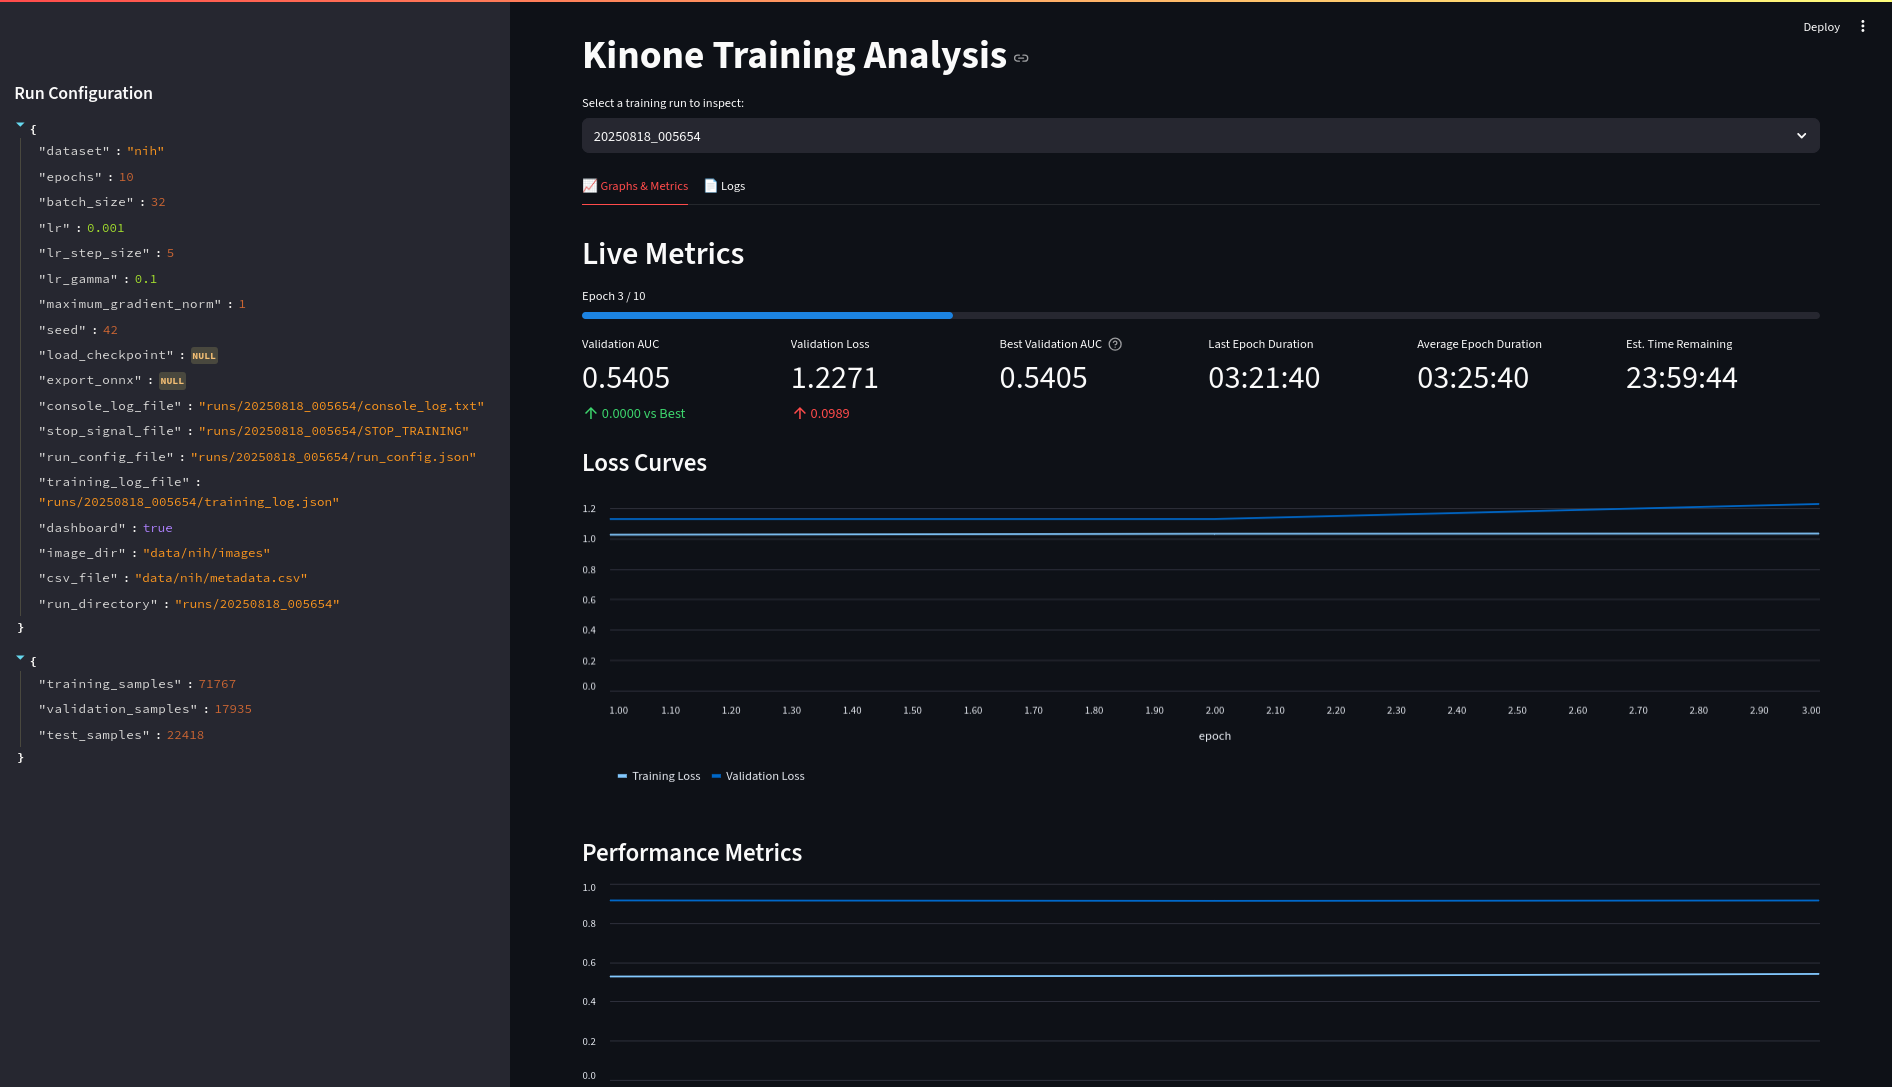
\includegraphics[width=0.7\textwidth]{dashboard}
  \caption{Kinone Dashboard}
  \label{fig:kinone_dashboard}
\end{figure}

\section{Verification and Testing Strategy}

In a system as complex as an automatic differentiation framework, correctness is not an incidental feature but the primary requirement. A subtle error in the gradient calculation for a single primitive operation can lead to catastrophic failures in model training that are exceedingly difficult to debug. Consequently, a rigorous and systematic verification strategy was a cornerstone of the Kinone project. The entire framework is underpinned by a comprehensive test suite that ensures the fidelity and reliability of every component, with a particular focus on the autograd engine.

\subsection{Unit Testing with Pytest}

The project employs a standard unit testing methodology using the Pytest framework. The test suite, located in the \texttt{tests/} directory, is organized to mirror the structure of the main source code. This modular approach ensures that every component of the framework, from data loaders to optimizers, is tested in isolation. Key areas covered by the unit tests include:

\begin{itemize}
    \item \textbf{Data Pipeline:} Verifying correct batching, shuffling, and data shapes from the \texttt{DataLoader}.
    \item \textbf{Loss Functions:} Ensuring that loss calculations are numerically correct and produce the expected gradients.
    \item \textbf{Optimizers:} Testing that parameter updates are applied correctly according to the specific algorithm's rules.
    \item \textbf{Module and Layer Functionality:} Confirming that model layers are constructed correctly and that state management (e.g., switching between training and evaluation modes) functions as expected.
\end{itemize}

While these tests are essential for verifying the high-level logic of the framework, the most critical part of the testing strategy is the specific method used to validate the correctness of the autograd engine itself.

\subsection{Gradient Verification via Finite Differences}

The correctness of the entire gradient-based learning process relies on the analytical gradients implemented in the \texttt{backward} method of each \texttt{Function} subclass. To verify these analytical implementations, a numerical approximation of the gradient is used as an independent ground truth. The chosen method for this numerical approximation is the finite-difference method.

Specifically, the project uses the second-order central-difference formula to estimate the partial derivative of a scalar function $f(\mathbf{x})$ with respect to a single component $x_i$ of its input vector $\mathbf{x}$:
\begin{equation}
    \frac{\partial f}{\partial x_i} \approx \frac{f(\mathbf{x} + h \mathbf{e}_i) - f(\mathbf{x} - h \mathbf{e}_i)}{2h}
    \label{eq:central_difference}
\end{equation}
where $\mathbf{e}_i$ is a standard basis vector with a one at the $i$-th position and zeros elsewhere, and $h$ is a small, finite step size (chosen as $10^{-3}$ for float32 precision). By iterating this calculation over all elements of the input tensor $\mathbf{x}$, we can construct a full numerical gradient, $\hat{\nabla}f(\mathbf{x})$.

A helper function, \texttt{finite\_difference\_gradients}, was implemented in \texttt{tests/utils.py} to automate this process for any given function and set of input tensors. This function became the core of the verification strategy for the autograd engine. For every single primitive operation implemented in Kinone, a dedicated test was written that follows this procedure:

\begin{enumerate}
    \item Instantiate one or more input \texttt{Tensor}s with \texttt{requires\_grad=True}.
    \item Apply the operation to these tensors to produce an output tensor.
    \item To obtain a scalar loss, a reduction (e.g., \texttt{mean()} or \texttt{sum()}) is applied to the output.
    \item The \texttt{backward()} method is called on the final scalar loss, which triggers the autograd engine to compute and populate the analytical gradients in the \texttt{.grad} attribute of the input tensors.
    \item Separately, the \texttt{finite\_difference\_gradients} utility is used to compute the numerical gradients for the same composite function.
    \item Finally, the analytical gradient computed by Kinone is compared to the numerical gradient using \texttt{numpy.allclose}, which checks for element-wise equality within a specified tolerance.
\end{enumerate}

This procedure was applied exhaustively to every operation, including element-wise functions, matrix multiplication, convolutions with various parameters (stride, padding, bias), pooling, and batch normalization. An example of a typical gradient test for a binary operation is shown in Listing \ref{lst:grad_test}.

\begin{lstlisting}[caption={Example of a gradient verification test for the \texttt{mul} operation.}, label={lst:grad_test}]
import numpy as np
from src.core.ops import mul
from src.core.tensor import Tensor
from tests.utils import assertion, finite_difference_gradients

def test_mul_grad():
  shape = (4, 4)
  a = Tensor(np.random.randn(*shape), requires_grad=True)
  b = Tensor(np.random.randn(*shape), requires_grad=True)
  
  # 1. Compute analytical gradients via Kinone's autograd
  mul(a, b).mean().backward()
  
  # 2. Compute numerical gradients via finite differences
  num_grad_a, num_grad_b = finite_difference_gradients(
    lambda x, y: (x * y).mean(), [a.data.copy(), b.data.copy()]
  )
  
  # 3. Assert that the two are close
  assertion(a.grad.data, num_grad_a)
  assertion(b.grad.data, num_grad_b)
\end{lstlisting}

This comprehensive, gradient-centric testing strategy provides a very high degree of confidence in the correctness of the framework's core engine. It ensures that any model built with Kinone will have mathematically correct gradients, forming a reliable foundation for all training and experimentation.

\section{Conclusion and Future Work}

This project set out with the ambitious goal of building a modern deep learning framework from first principles, driven by the motivation to create a system that is transparent, educational, and algorithmically explicit. By adhering to a philosophy of implementing every core component from scratch using only NumPy, the Kinone framework has successfully met these objectives. This final section summarizes the key achievements of the project, reflects on the valuable insights gained during its development, and outlines promising directions for future work.

\subsection{Summary of Project}

Over the course of this project, a complete, end-to-end deep learning ecosystem was successfully engineered. The key accomplishments can be summarized as follows:

\begin{itemize}
    \item \textbf{A Functional Autograd Engine:} A robust reverse-mode automatic differentiation engine was implemented. It dynamically builds a computational graph and correctly computes gradients for complex, composite functions, forming the reliable core of the entire framework.

    \item \textbf{A Modular Library of Neural Network Primitives:} A comprehensive set of standard neural network operations, layers, and activation functions was developed. This modular library enables the flexible construction of a wide variety of network architectures.

    \item \textbf{Implementation of State-of-the-Art Architectures:} The framework's capabilities were validated through the successful implementation of complex, canonical models, including the ResNet and EfficientNet families. This demonstrated that the abstractions were powerful enough to support modern deep learning research.

    \item \textbf{An End-to-End Workflow:} Kinone provides a complete workflow for a machine learning project, from data ingestion and preparation with a custom data pipeline to model training with multiple optimization algorithms and finally to evaluation.

    \item \textbf{Verified Correctness:} The correctness of the framework, particularly the critical gradient calculations, was systematically verified through a rigorous testing suite that benchmarked all analytical gradients against numerical finite-difference approximations.

    \item \textbf{Advanced Tooling for Interoperability and Analysis:} The framework is augmented with powerful tools, including an ONNX exporter for model deployment and a live Streamlit dashboard for real-time training monitoring, elevating it from a simple library to a more complete development environment.
\end{itemize}

\subsection{Key Learnings}

The process of building Kinone from the ground up provided numerous invaluable insights that are often abstracted away by high-level libraries. A primary lesson was a deeper, more intuitive understanding of the backpropagation algorithm; implementing the backward pass for diverse operations like broadcasting, convolution, and batch normalization solidified the theoretical concepts in a practical context. The project also highlighted the nuances of numerical stability, particularly in the implementation of activation and loss functions. Furthermore, it fostered an appreciation for the software engineering patterns that make deep learning frameworks both flexible and scalable, such as the modular design, the separation of operations from layers, and the importance of a clean and consistent API.

\subsection{Future Directions}

While Kinone has achieved its initial goals, it also serves as a strong foundation for many potential extensions and improvements. Future work could proceed in several promising directions:

\begin{itemize}
    \item \textbf{Performance Optimization:} The most significant limitation of the current framework is its reliance on a pure Python and NumPy backend, which makes it computationally slow. A major avenue for future work would be to integrate a high-performance backend. This could involve using a Just-In-Time (\acronym{jit}) compiler like Numba to accelerate critical loops, or more ambitiously, creating an alternative backend that translates the computational graph to a system like JAX or CuPy to enable seamless GPU acceleration.

    \item \textbf{Expanding the Operator Set:} The current library of operations could be expanded to support a wider range of model architectures. Key additions would include operations required for Transformer models, such as multi-head self-attention, and operations for recurrent neural networks (\acronym{rnn}s), like \acronym{lstm} or \acronym{gru} cells.

    \item \textbf{Advanced Framework Features:} The framework could be enhanced with more sophisticated features found in production libraries. This might include implementing higher-order differentiation (the ability to compute gradients of gradients), a more diverse set of learning rate schedulers, and built-in support for model checkpointing and automated experiment tracking.

    \item \textbf{Embedded Deployment and Model Quantization:} A particularly exciting direction would be to bridge the gap between training and deployment on edge devices. The existing ONNX export capability is the first step in this process. A future project could build a pipeline that takes the exported ONNX model, applies post-training quantization to reduce its size and computational requirements (e.g., converting float32 weights to int8), and then deploys it to an embedded \acronym{ai} platform. Using a toolchain like Vitis \acronym{ai}, the quantized model could be compiled for deployment on System-on-Chip (\acronym{soc}) boards with programmable logic, such as the AMD-Xilinx Kria KV260 Vision AI Starter Kit, enabling efficient, low-latency inference directly on hardware. This would complete the full lifecycle from theoretical implementation to real-world application.
\end{itemize}

In its current state, Kinone stands as a testament to the power of building from first principles. It is a robust, well-tested, and transparent framework that successfully achieves its goal of demystifying the core mechanics of deep learning.

\section{Code Availability}
The complete source code for the Kinone framework, including all experiments and testing scripts detailed in this report, is publicly available on GitHub: \url{https://github.com/pseudofractal/Kinone/}.

\pagebreak
\begin{thebibliography}{1}

\bibitem{paszke2019pytorch}
A.~Paszke, S.~Gross, F.~Massa, A.~Lerer, J.~Bradbury, G.~Chanan, T.~Killeen, Z.~Lin, N.~Gimelshein, L.~Antiga, et~al., ``Pytorch: An imperative style, high-performance deep learning library,'' in {\em Advances in Neural Information Processing Systems}, pp.~8026--8037, 2019.

\bibitem{rumelhart1986learning}
D.~E. Rumelhart, G.~E. Hinton, and R.~J. Williams, ``Learning representations by back-propagating errors,'' {\em Nature}, vol.~323, no.~6088, pp.~533--536, 1986. [4, 11, 15, 17]

\bibitem{lecun1998gradient}
Y.~LeCun, L.~Bottou, Y.~Bengio, and P.~Haffner, ``Gradient-based learning applied to document recognition,'' {\em Proceedings of the IEEE}, vol.~86, no.~11, pp.~2278--2324, 1998. [26, 41]

\bibitem{ioffe2015batch}
S.~Ioffe and C.~Szegedy, ``Batch normalization: Accelerating deep network training by reducing internal covariate shift,'' in {\em International Conference on Machine Learning}, pp.~448--456, PMLR, 2015. [1, 2, 5, 9, 18]

\bibitem{hinton2012neural}
G.~Hinton, ``Neural networks for machine learning, lecture 6e.'' Coursera, 2012. [22, 23, 24]

\bibitem{kingma2014adam}
D.~P. Kingma and J.~Ba, ``Adam: A method for stochastic optimization,'' {\em arXiv preprint arXiv:1412.6980}, 2014. [6, 20, 25, 29]

\bibitem{he2016deep}
K.~He, X.~Zhang, S.~Ren, and J.~Sun, ``Deep residual learning for image recognition,'' in {\em Proceedings of the IEEE Conference on Computer Vision and Pattern Recognition}, pp.~770--778, 2016. [30, 32, 40]

\bibitem{tan2019efficientnet}
M.~Tan and Q.~V. Le, ``Efficientnet: Rethinking model scaling for convolutional neural networks,'' in {\em International Conference on Machine Learning}, pp.~6105--6114, PMLR, 2019. [3, 10, 13, 14]

\bibitem{hu2018squeeze}
J.~Hu, L.~Shen, and G.~Sun, ``Squeeze-and-excitation networks,'' in {\em Proceedings of the IEEE Conference on Computer Vision and Pattern Recognition}, pp.~7132--7141, 2018. [19, 21, 31, 38]

\end{thebibliography}

\end{document}
